\documentclass[a4paper,12pt]{article}[abntex2]
\bibliographystyle{abntex2-alf}
\usepackage{siunitx} % Fornece suporte para a tipografia de unidades do Sistema Internacional e formatação de números
\usepackage{booktabs} % Melhora a qualidade das tabelas
\usepackage{tabularx} % Permite tabelas com larguras de colunas ajustáveis
\usepackage{graphicx} % Suporte para inclusão de imagens
\usepackage{newtxtext} % Substitui a fonte padrão pela Times Roman
\usepackage{ragged2e} % Justificação de texto melhorada
\usepackage{setspace} % Controle do espaçamento entre linhas
\usepackage[a4paper, left=3.0cm, top=3.0cm, bottom=2.0cm, right=2.0cm]{geometry} % Personalização das margens do documento
\usepackage{lipsum} % Geração de texto dummy 'Lorem Ipsum'
\usepackage{fancyhdr} % Customização de cabeçalhos e rodapés
\usepackage{titlesec} % Personalização dos títulos de seções
\usepackage[portuguese]{babel} % Adaptação para o português (nomes e hifenização
\usepackage{hyperref} % Suporte a hiperlinks
\usepackage{indentfirst} % Indentação do primeiro parágrafo das seções
\sisetup{
  output-decimal-marker = {,},
  inter-unit-product = \ensuremath{{}\cdot{}},
  per-mode = symbol
}
\DeclareSIUnit{\real}{R\$}
\newcommand{\real}[1]{R\$#1}
\usepackage{float} % Melhor controle sobre o posicionamento de figuras e tabelas
\usepackage{footnotehyper} % Notas de rodapé clicáveis em combinação com hyperref
\hypersetup{
    colorlinks=true,
    linkcolor=black,
    filecolor=magenta,      
    urlcolor=cyan,
    citecolor=black,        
    pdfborder={0 0 0},
}
\usepackage[normalem]{ulem} % Permite o uso de diferentes tipos de sublinhados sem alterar o \emph{}
\makeatletter
\def\@pdfborder{0 0 0} % Remove a borda dos links
\def\@pdfborderstyle{/S/U/W 1} % Estilo da borda dos links
\makeatother
\onehalfspacing
\setlength{\headheight}{14.49998pt}

\begin{document}

\begin{titlepage}
    \centering
    \vspace*{1cm}
    \Large\textbf{INSPER – INSTITUTO DE ENSINO E PESQUISA}\\
    \Large \textbf{ECONOMIA}\\
    \vspace{1.5cm}
    \Large\textbf{Atividade Prática Superviosionada IV}\\
    \textbf{Macroeconomia Internacional}\\
    \vspace{1.5cm}
    Prof. Gino Olivares\\
    Prof. Auxiliar Victor Dias \\
    \vfill
    \normalsize
    Fabrizio Antonini Ripoli, \href{mailto:fabrizioar@al.insper.edu.br}{fabrizioar@al.insper.edu.br}\\
    Hicham Munir Tayfour, \href{mailto:hichamt@al.insper.edu.br}{hichamt@al.insper.edu.br}\\
    4º Período - Economia B\\
    \vfill
    São Paulo\\
    Maio/2024
\end{titlepage}

\newpage
\tableofcontents
\thispagestyle{empty} % This command removes the page number from the table of contents page
\newpage
\setcounter{page}{1} % This command sets the page number to start from this page
\justify
\onehalfspacing

\pagestyle{fancy}
\fancyhf{}
\rhead{\thepage}

\section{\textbf{Situação 1}}

Figura~\ref{fig:AADD La}

\begin{figure}[H]
    \centering
    \caption{AA-DD} 
    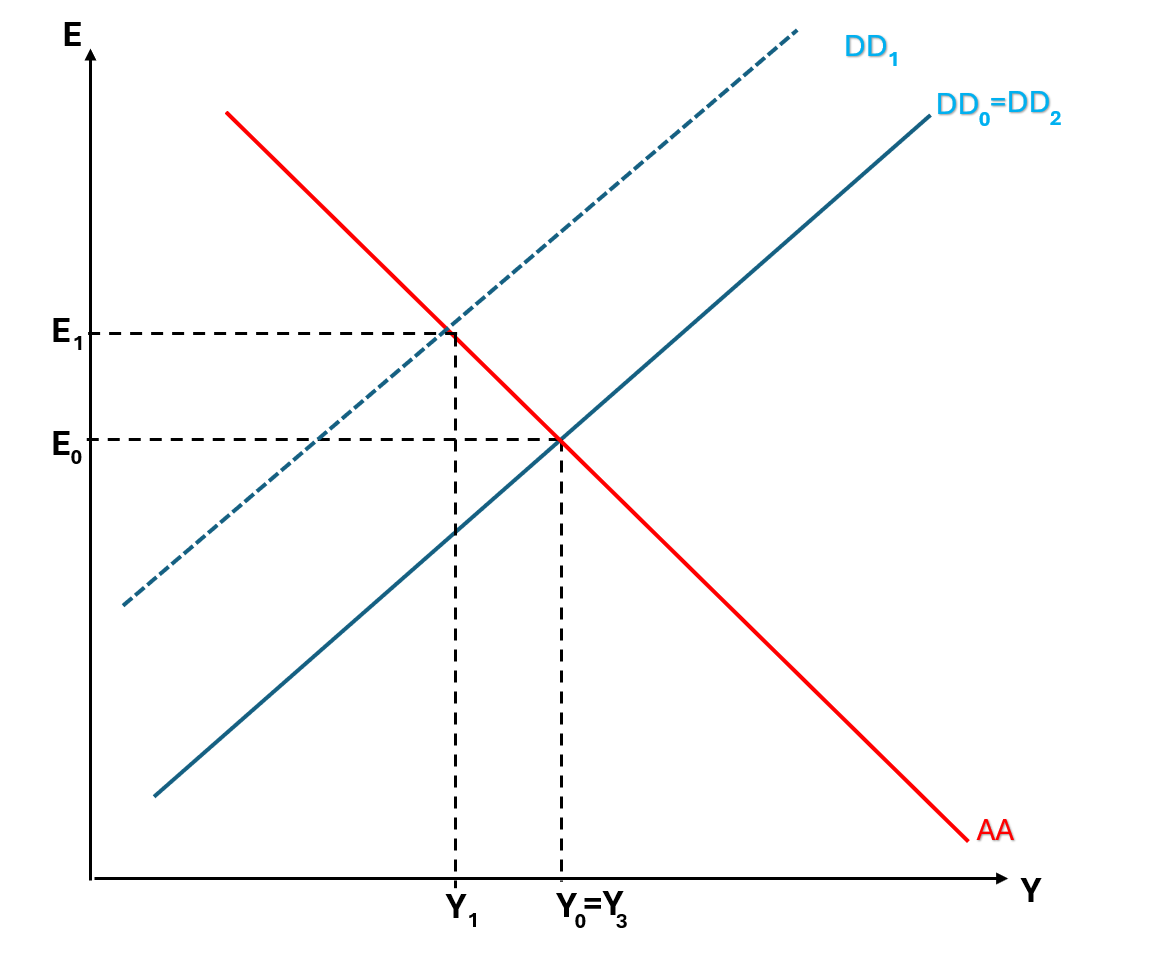
\includegraphics[width=0.7\textwidth]{4º Período/Macroeconomia Internacional/APS 4 Macro Int/AA-DD L(a).png}
    \label{fig:AADD La}
    
    \footnotesize{Fonte: Elaborado pelos autores.}
    \end{figure}

\subsection{\textbf{Letra A}}
Uma queda da confiança do consumidor doméstico afeta o mercado de bens , logo a curva DD será afetada por esse choque. Há um desequilíbrio no mercado de bens devido a uma redução do consumo. Esse redução da demanda por bens reduz o produto.

\subsection{\textbf{Letra B}}

 Essa redução do PIB \((Y_0>Y_1\)), impactando no mercado monetário, deslocando demanda por moeda para um nível inferior devido ao PIB menor \(L(Y_1;R)<L(Y_0;R)\). A queda da demanda por moeda dada a mesma oferta de moeda gera uma redução da taxa de juros doméstica \(R_0 \to R_1\) e como consequência o câmbio deprecia \(E_0 \to E_1\).

\newpage
Figura~\ref{fig:Moeda La}

\begin{figure}[H]
    \centering
    \caption{Mercado Monetário e Cambial} 
    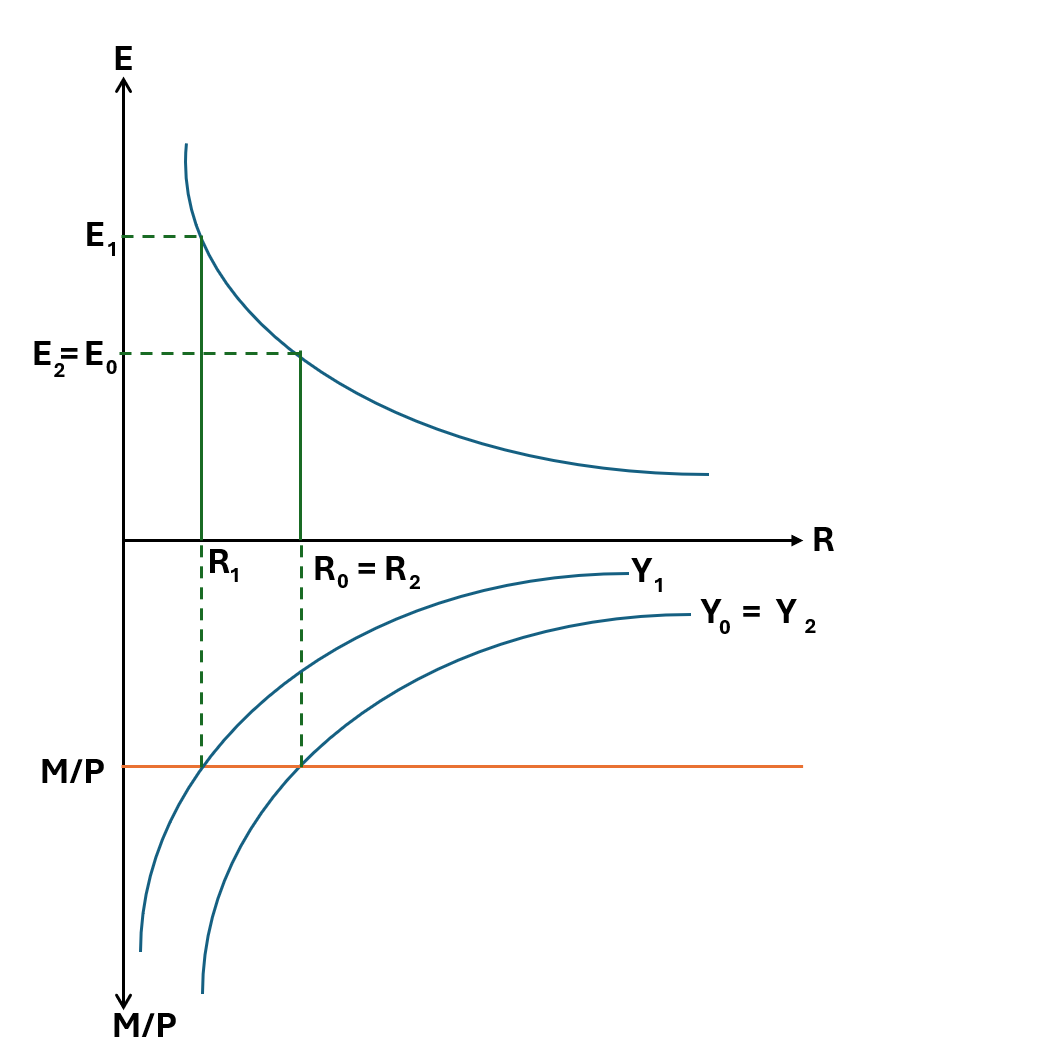
\includegraphics[width=0.7\textwidth]{4º Período/Macroeconomia Internacional/APS 4 Macro Int/Merc. Mont L(a).png}
    \label{fig:Moeda La}
    
    \footnotesize{Fonte: Elaborado pelos autores.}
    \end{figure}
    
\subsection{\textbf{Letra C}}

Dada a origem do choque no mercado de bens, o ideal seria uma política fiscal expansionista para ocupar o "espaço" deixado pela redução do consumo para que o nível de câmbio seja mantido igual ao que era antes do choque. Para ajustar o mercado monetário a um novo equilíbrio no mercado de bens, o câmbio teria que ser apreciado para que o produto voltasse a ser o original (não ideal).
Nesse sentido, considerando uma política fiscal que aumenta os gastos governamentais, a composição do PIB seria tal que o consumo seria menor que o de origem e o gasto do governo maior.

\subsection{\textbf{Letra D}}

Agora, considerando uma curva XX, para manter o equilíbrio da economia no mesmo nível de conta corrente, será necessário adotar uma política monetária contracionista. Assim, haverá uma compensação da apreciação do câmbio pela diminuição do produto na balança comercial.

\section{\textbf{Situação 2}}
\begin{figure}[H]
    \centering
    \caption{AA-DD} 
    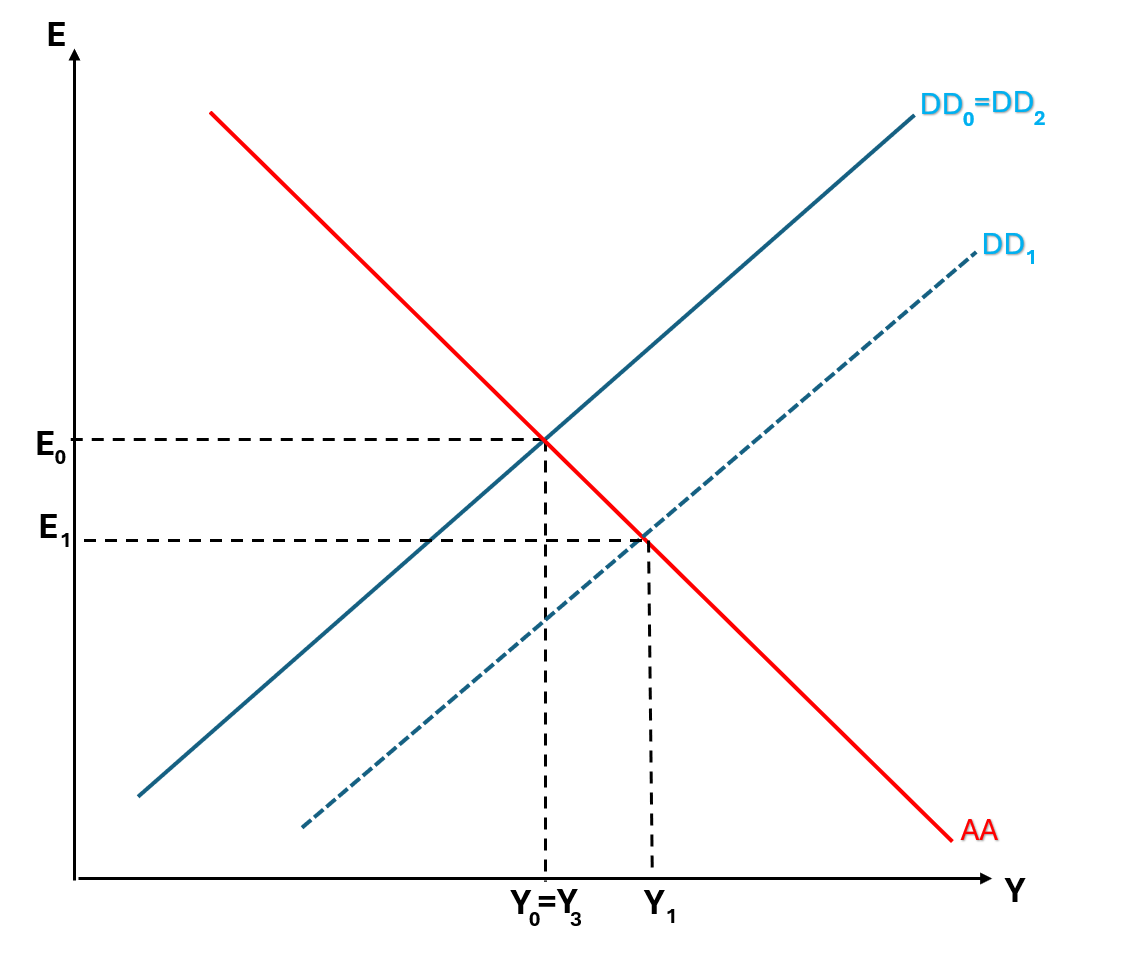
\includegraphics[width=0.7\textwidth]{4º Período/Macroeconomia Internacional/APS 4 Macro Int/AA-DD L(b).png}
    \label{fig:AADD Lb}
    
    \footnotesize{Fonte: Elaborado pelos autores.}
    \end{figure}
    


\subsection{\textbf{Letra A}}
Uma melhoria no ambiente de negócios local afeta o mercado de bens , logo a curva DD será afetada por esse choque. Há um desequilíbrio no mercado de bens devido a um aumento do investimento. Esse aumento da demanda por bens eleva o produto.

\subsection{\textbf{Letra B}}

 Esse aumento do PIB, impacta no mercado monetário, deslocando demanda por moeda para um nível superior devido ao PIB maior . O aumento da demanda por moeda dada a mesma oferta de moeda gera um aumento da taxa de juros doméstica  e como consequência o câmbio aprecia .

 \begin{figure}[H]
    \centering
    \caption{Mercado Monetário e Cambial} 
    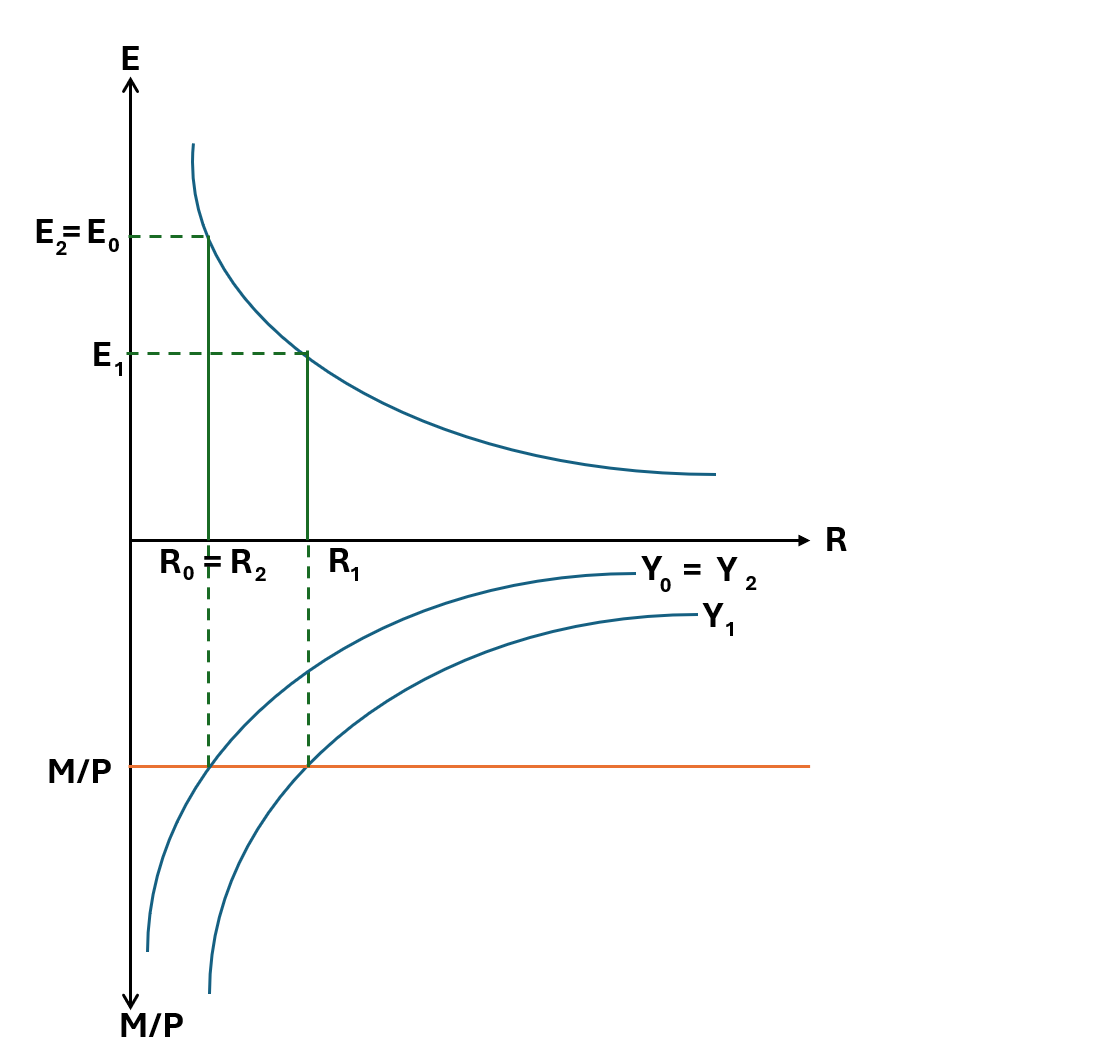
\includegraphics[width=0.7\textwidth]{4º Período/Macroeconomia Internacional/APS 4 Macro Int/Merc. Mont L(b).png}
    \label{fig:Moeda Lb}
    
    \footnotesize{Fonte: Elaborado pelos autores.}
    \end{figure}

\subsection{\textbf{Letra C}}

A mesma lógica de 2.3 pode ser aplicada aqui. O ideal seria uma política fiscal de retração para livrar "espaço" ocupado pelo aumento do investimento para que o nível de câmbio seja mantido igual ao que era antes do choque. Nesse cenário, o produto seria composto por mais investimento e menos gastos governamentais do que anteriormente.

\subsection{\textbf{Letra D}}
 Considerando uma curva XX, para manter o equilíbrio da economia no mesmo nível de conta corrente, será necessário adotar uma política monetária expansionista. Assim, haverá uma compensação da depreciação do câmbio pela aumento do produto na balança comercial.

\section{\textbf{Situação 3}}
\begin{figure}[H]
    \centering
    \caption{AA-DD} 
    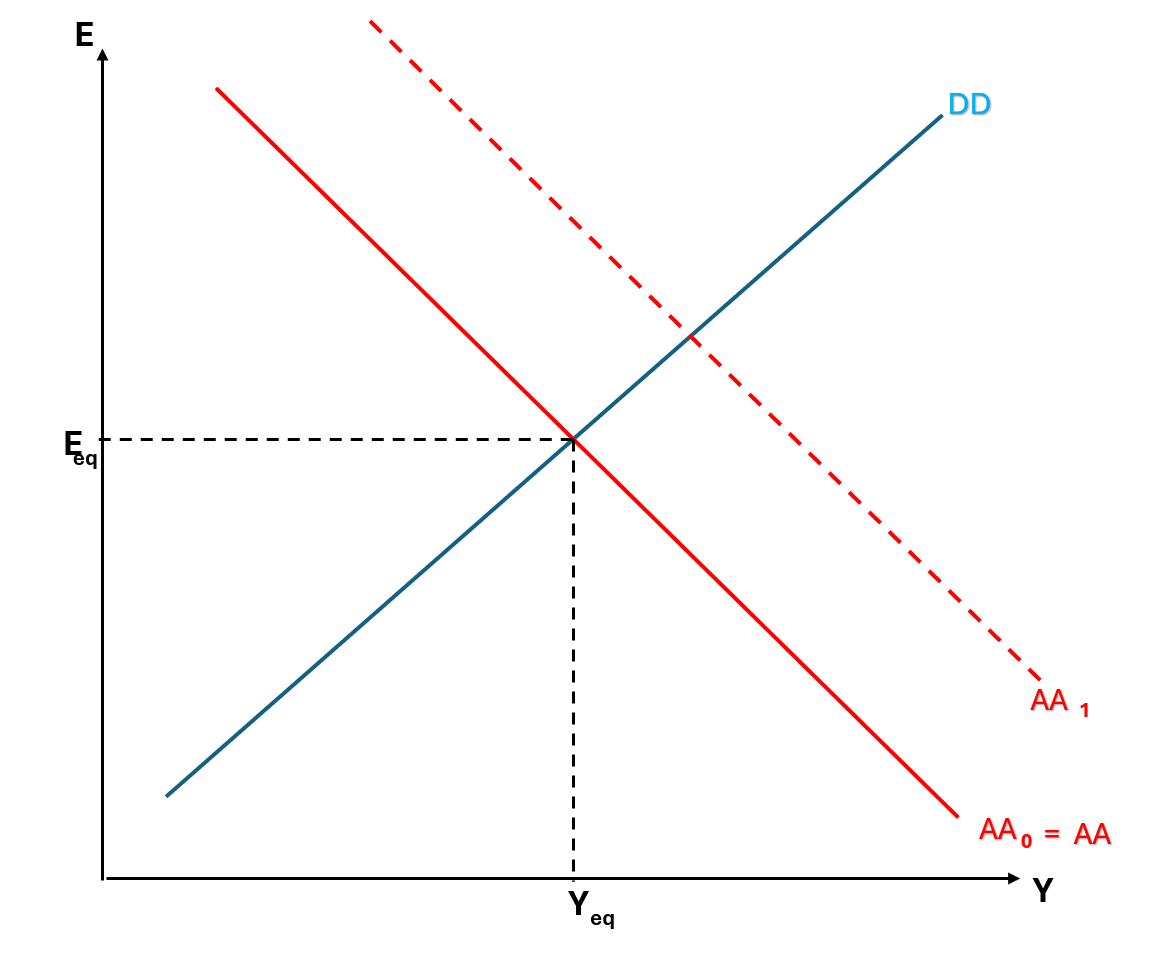
\includegraphics[width=0.7\textwidth]{4º Período/Macroeconomia Internacional/APS 4 Macro Int/AA-DD L(c).png}
    \label{fig:AADD L}
    
    \footnotesize{Fonte: Elaborado pelos autores.}
    \end{figure}

\subsection{\textbf{Letra A}}

No mercado monetário, o aumento da taxa de juros externa torna mais vantajoso investir no exterior do que dentro do país, tudo o mais constante. Isso faz a demanda por moeda externa aumentar, fazendo a moeda doméstica depreciar em relação à externa.

\subsection{\textbf{Letra B}}

Essa depreciação do câmbio faz com que o mercado externo queira comprar os produtos nacionais, aumentando as exportações. Isso melhora a conta corrente, aumentando o nível de produto.

\begin{figure}[H]
    \centering
    \caption{Mercado Monetário e Cambial} 
    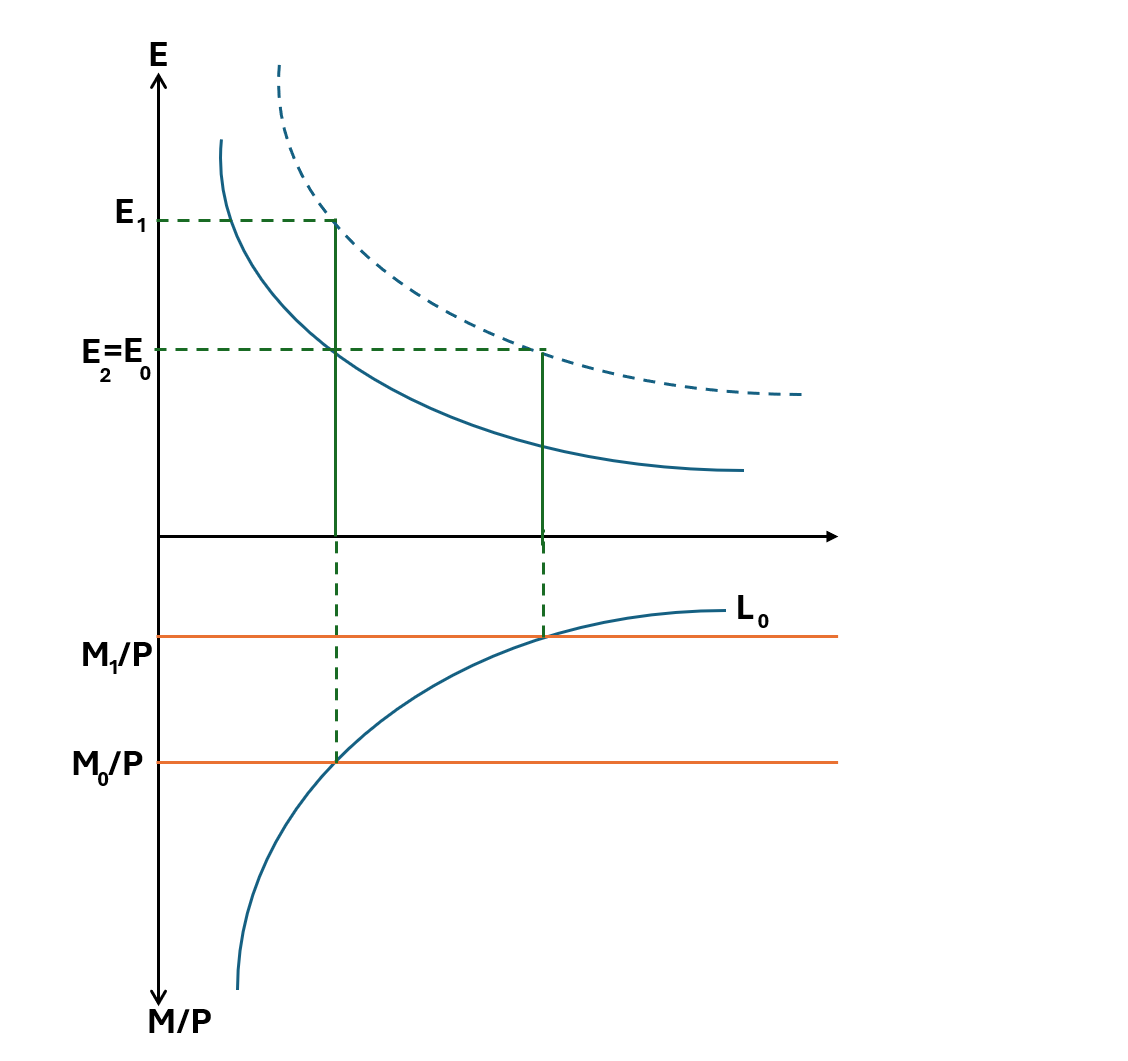
\includegraphics[width=0.7\textwidth]{4º Período/Macroeconomia Internacional/APS 4 Macro Int/Merc. Mont L(c).png}
    \label{fig:Moeda L}
    
    \footnotesize{Fonte: Elaborado pelos autores.}
    \end{figure}

\subsection{\textbf{Letra C}}
O ideal seria uma política monetária de contração para que o nível de câmbio seja mantido igual ao que era antes do choque. Nesse cenário, o produto seria composto pelos mesmo itens, pois a mudança que aconteceu no produto por causa da alteração do câmbio seria neutralizada pelo ajuste do câmbio pela política monetária.

\subsection{\textbf{Letra D}}
Neste caso, considerando uma curva XX, se desejarmos permanecer na interseção da curva XX com a curva AA após o choque, será necessário adotar uma política fiscal expansionista. Isso resultará em uma taxa de câmbio mais depreciada, mas também em um produto maior.

Se desejamos voltar ao nível inicial de produto e taxa de câmbio, mantendo a curva XX no mesmo nível, será necessário adotar uma política monetária contracionista, o que deslocará a curva AA ao longo da XX.

\section{\textbf{Situação 4}}
\begin{figure}[H]
    \centering
    \caption{AA-DD} 
    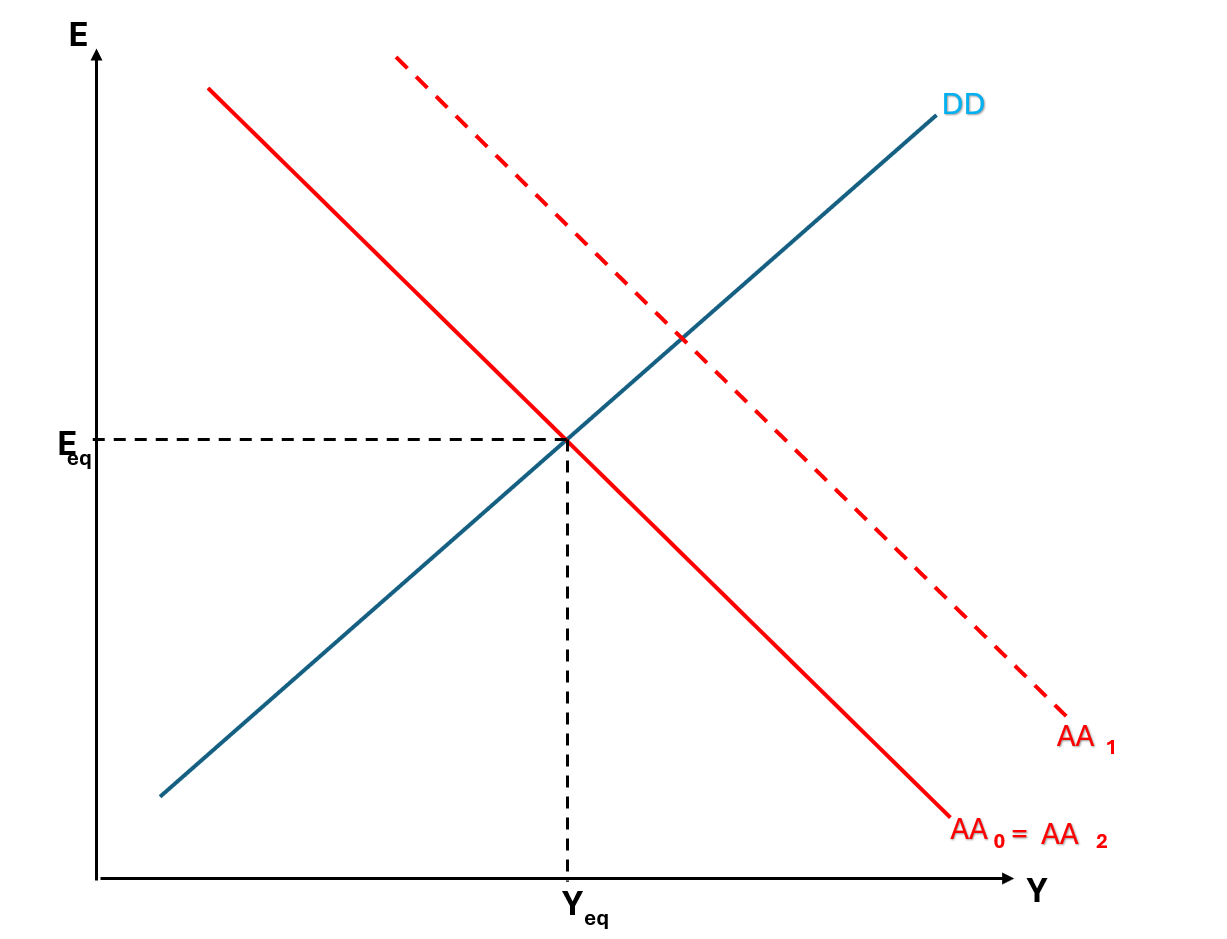
\includegraphics[width=0.7\textwidth]{4º Período/Macroeconomia Internacional/APS 4 Macro Int/AA-DD L(d).png}
    \label{fig:AADD L}
    
    \footnotesize{Fonte: Elaborado pelos autores.}
    \end{figure}

\subsection{\textbf{Letra A}}

No mercado de ativos, a redução de demanda por moeda causa aumento do preço do juros, o que deprecia o câmbio, uma vez que investir nos títulos nacionais não é mais tão vantajoso como costumava ser.

\subsection{\textbf{Letra B}}

\begin{figure}[H]
    \centering
    \caption{Mercado Monetário e Cambial} 
    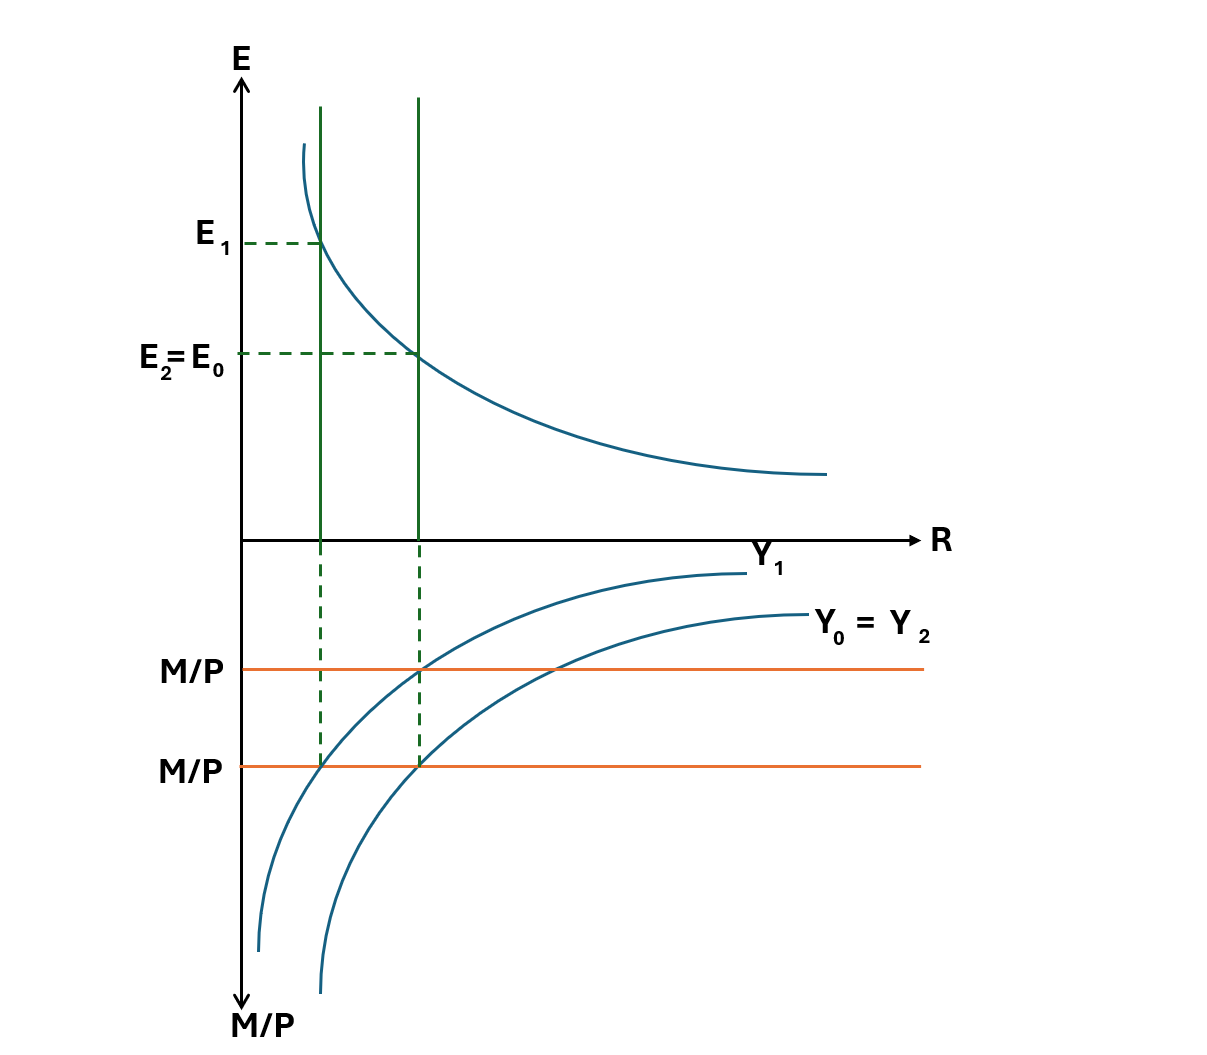
\includegraphics[width=0.7\textwidth]{4º Período/Macroeconomia Internacional/APS 4 Macro Int/Merc. Mont L(d).png}
    \label{fig:Moeda L}
    
    \footnotesize{Fonte: Elaborado pelos autores.}
    \end{figure}


Do mesmo jeito da situação anterior, a depreciação do câmbio faz com que o mercado externo queira comprar os produtos nacionais, aumentando as exportações. Isso melhora a conta corrente, aumentando o nível de produto.

\subsection{\textbf{Letra C}}

Dada a origem do choque no mercado de ativos, o ideal seria uma política monetária contracionista
para aliviar as pressões no câmbio causadas pela diminuição da demanda por moeda. Nesse caso, a composição do pIB não será alterada.

\subsection{\textbf{Letra D}}
Para manter a curva XX no mesmo resultado, tanto em termos de política fiscal quanto monetária, será o mesmo procedimento da Situação 3, considerando o impacto do choque na curva AA. A diferença estará nos motivos para realizar esses ajustes.


\end{document}